\chapter{Analogue to Digital Converter}

Before discussing an Analogue to Digital Converter (ADC), first consider the simple GPIO pin configured as an input. 
The pin "reads" the voltage applied to it and produces a binary number (a 1 or a 0) which indicates whether the applied voltage is a high or low. Technically this GPIO pin is an analogue to digital converter: it takes an analogue voltage and produces a binary number representing that voltage. 
However, having only 1 bit to represent the voltage applied to the pin means that we get a very poor approximation of the voltage. 
For example, we cannot tell the different between 2 V and 3 V being applied to the pin: both of those voltages are considered a logic 1. 
For this reason we do not typically refer to a GPIO pin as an ADC, rather we refer to it as a digital input.

The term ADC is typically reserved for a peripheral inside the microcontroller which has the ability to provide a much higher resolution and higher accuracy numerical approximation of the applied voltage. 
While a GPIO pin is able to digitise the voltage to only 1 bit, the ADC can typically digitise the voltage to many bits. 

\section{Transfer Function}
A transfer function is the mathematical relationship between the input voltage and the output value of the ADC.
Different ADCs with different architectures have different transfer functions. What is discussed here is the transfer function for the ADC used inside our STM32F051 microcontroller. 

First note that because we have a finite number of possible numberical outputs of the ADC which must map to the full voltage range which the ADC operates over, each numerical output of the ADC corresponds to a \emph{range} of input voltages. 
The number of bits determines the number of possible numerical outputs or \emph{quantization intervals} which the system has. A quantisation interval is an input voltage range which produces a certain digital output. The supply rail is divided up into \(N = 2^M\) quantisation intervals where \(M\) is the number of bits of the ADC. 
A change of one \emph{least significant bit} of the value of the digital output corresponds to going to the next quantisation interval. 

As stated, there are \(N\) quantisation intervals. An ADC will typically digitise voltages between \SI{0}{\volt} (ground), and some upper limit \(V_{ref}\), which is often set to the supply voltage of the microcontroller. If we have a reference voltage \(V_{ref}\) volts, then each quantisation interval is \(Q = \frac{V_{ref}}{N}\) volts wide.
We realise that each digital output corresponds to a \emph{range} of input voltages. How big is the range? Seeing as the ADC can only work in multiple of a lsb, the range must be one lsb wide. 
The ADC in the STM32 has been structured such that the midpoint of the range which produced a digital output of \(k\) is equal to \(V_{k} = k \times \frac{V_{ref}}{N}\). 
Hence, the range of input voltage corresponding to a digital output of \(k\) is: \(kQ - 0.5Q\) to \(kQ + 0.5Q\). Intuitively, this is \(k\) lsbs with half a lsb uncertainty each way. 

It must be stressed that different ADC architectures may have a slightly different transfer function (the relationship between the input voltage and output digital value). 
The transfer function discussed above is the one implemented by our STM32.

\begin{figure}
  \centering
  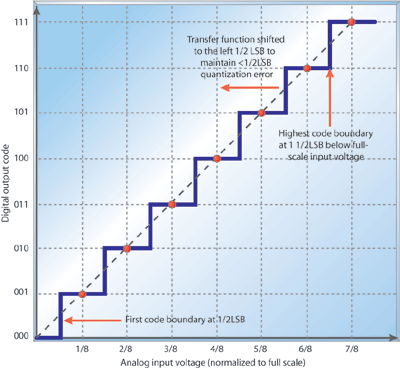
\includegraphics[width=0.5\textwidth]{adc_transfer.png}
  \caption{Example graph of ADC transfer function for 3-bit ADC.}
  \label{fig:adc-transfer-graph}
\end{figure}


\section{Example Calculation}
For an example of this, let's consider the case of a 3 bit ADC running off of a \(V_{ref}\) of \SI{4.0}{\volt}. One lsb has a value of \(V_{lsb} = \frac{\SI{4}{\volt}}{2^3} = \SI{0.5}{\volt}\).
Half a lsb, or the uncertainty around each value is hence \(\frac{\SI{0.5}{\volt}}{2} = \SI{0.25}{\volt}\)
Hence, the input voltage range for a digital output of \(k\) is equal to \((k \times \SI{0.5}{\volt}) \pm \SI{0.25}{\volt}\).
All input/output values for this example ADC are shown in \autoref{tab:3-bit-adc}. \\

\begin{table}[t]
\centering
\begin{tabu}{c | c | l}
  Output & Midpoint (V) & Voltage Range (V)\\
      \hline
      000 & 0 & below 0.25 \\
      001 & 0.5 & 0.25 to 0.75 \\
      010 & 1.0 & 0.75 to 1.25 \\
      011 & 1.5 & 1.25 to 1.75\\
      100 & 2.0 & 1.75 to 2.25\\
      101 & 2.5 & 2.25 to 2.75 \\
      110 & 3.0 & 2.75 to 3.25 \\
      111 & 3.5 & 3.25 and above\\
\end{tabu}
\caption{Numerical output vs applied voltage band for a 3 bit ADC running off of \SI{4}{\volt}.}
\label{tab:3-bit-adc}
\end{table}

We see, therefore, that in general to calculate the corresponding input voltage range for a certain digital output:
\begin{enumerate}
  \item Calculate the size of each quantisation interval (aka: value of one lsb): \(Q = \frac{V_{ref}}{2^M}\) volts.
  \item The output \(k\) means we go up \(k\) quantisation intervals to the midpoint: \(kQ\)
  \item Add the uncertainty each way, half a lsb: \(\pm 0.5Q\)
\end{enumerate}

\section{ADC errors and calibration}
Inside the STM32F051 is a Switched Capacitor Successive Approximation Register Analogue to Digital Converter (SC SAR ADC). 
This ADC architecture consists of an array of capacitors, which can be selectively switched to GND or \(V_{ref}\). 
Each capacitor has a binary relationship to the next one, meaning that it's half the size. 
In other words, the first cap has a value of \(C\), the second has a value of \(\frac{C}{2}\), the third has a value of \(\frac{C}{4}\), then \(\frac{C}{8}\) etc.
The total capacitance of the array is typically a few picofarads. 
The ADC first goes through a \emph{sample} phase whereby it charges all of the capacitors up to the input voltage. It then disconnects the array of capacitors from the input voltage and goes through the process of approximating the voltage by switching the configuration of the capacitors and comparing the resultant voltage to a fixed voltage using an internal \emph{comparator}. This layout is shown in \autoref{fig:adc-component-level}. 

\begin{figure}
\centering
\includegraphics[page=5, clip=true, trim=75 360 75 280, width=\textwidth]{CD00211314.pdf}
% left, bottom, right, top
\caption{Internal workings of a SC SAR ADC. Note the analogue components: capacitors and comparator.}
\label{fig:adc-component-level}
\end{figure}

The key realisation you should take away from this is that an ADC involves the use of analogue components, specifically the capacitors which need to have precise values, and the comparator which ideally will have no input current and no input offset voltage. However, these being analogue components are NOT ideal. The capacitors will not be perfectly matched and the comparator will have some input offset voltage and input current.

The implication of this is that the ADC will not perform perfectly. The quantisation interval which we calculate under the case for a perfect ADC will probably not be how the ADC actually performs.
There are a few types of errors which an ADC suffers from including gain error, offset error, differential nonlinearity error, integral nonlinearity error, missing codes and duplicate codes. 

The one which I'd like to focus on is offset error. Offset error means that the transfer function is either advanced such that it outputs a higher digital output than it should or delayed such that it outputs a lower digital output than it should. 
This is shown graphically (and very exaggerated) in \autoref{fig:adc-offset-error}. Naturally, this is bad as it means that actual applied voltage corresponding to a certain digital output is not what we expect it to be. 

We have noticed the case of the positive offset error when working with our ADC. We notice that when turning our pot fully on (ie: going to the maximum value on the analogue input axis) we see that the digital output does not go all the way to the maximum value. Typically this error is small, but it would still be preferable to remove it if possible.\\

Fortunately the ADC has a calibration function which attempts to remove this error. I don't know exactly how it works inside, but I suspect that it connects the analogue input to a known reference voltage, performs a conversion and calculates the difference between the expected digital output and the actual digital output. It then adds or subtracts this offset amount from the digital output every time a conversion is done.

ADC calibration can be performed by setting the ADCAL bit in the ADC Control Register high. This starts the calibration procedure. You must then wait for this bit to be cleared by hardware which indicates that the cal procedure is complete and the ADC can be used. For full instructions, see section 13.4.1 of the reference manual. 

\begin{figure}
  \centering
  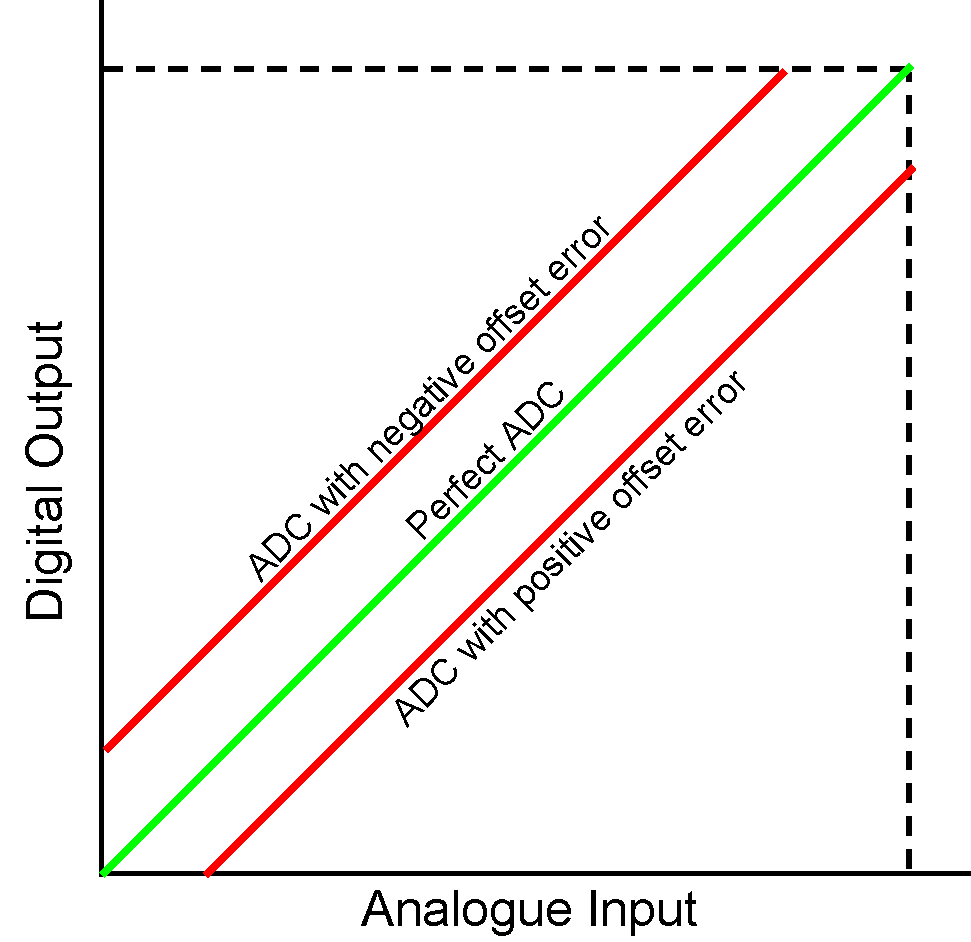
\includegraphics[width=0.7\textwidth]{adc-offset-error.pdf}
  \caption{Perfect ADC transfer function in green with no offset error. Transfer functions in red with positive or negative offset errors. Note firstly that these are greatly exaggerated errors from what is usual. A typical uncalibrated error for our ADC will be 1 or 2 percent. Note also that these transfer functions are not smooth lines in reality, they are actually made up of hundreds or thousands of quantisation intervals which are not shown here.}
  \label{fig:adc-offset-error}
\end{figure}


That concludes the overview of what an ADC is and how it works inside. We will now consider how to configure and use the ADC on our STM32.

\section{Using the ADC}
\subsection{Enabling}
Before the ADC peripheral can be used, it should be enabled. Two steps are required: 
\begin{enumerate}
\item Externally activating the ADC by providing clock to the peripheral by setting the corresponding bit in the RCC\_APB2ENR
\item Internally activating the ADC by setting the ADEN bit in the ADC\_CR
\end{enumerate}

After setting the ADEN bit, the ADC will take some time to power on. Once the ADEN bit has been set, you should wait until the ADRDY flag in the ADC\_ISR has gone high before you attempt to do anything with the ADC. 

\subsection{Channel}
The ADC is not limited to just reading from one fixed pin; it can select which pin to use from a number of possible sources, or \emph{channels}.
The ADC\_CHSELR register controls which channel is selected. On our device there are 10 different pins which can be selected for use as an ADC channel. In order to see which ADC channel a pin corresponds to, consult Table 13 of the Datasheet. This table shows which ADC channel a pin is connected to in the "Additional functions" column. For example, PB1 is connected to ADC channel 9.

\emph{Be careful not to set multiple channels in the ADC\_CHSELR simultaneously. If you do this, the ADC will scan through each of the channels. Unless you know what you're doing, this is probably not what you want and it will confuse you.}

\subsection{Pin Mode}
We know that by default a pin will operate in \emph{Input} mode. That is, it will digitise the applied voltage to a 1 bit number which will set/clear a bit in the GPIOx\_IDR. The component which does the digitising is the Schmitt trigger. 

This is not how we want the pin to function when using an ADC. When we want to use a pin as an ADC channel, we want the raw analogue voltage to be passed on to the ADC for digitising. In order to achieve this, the pin should be put into \emph{Analogue} mode. Here, the Schmitt trigger is disabled and the pin is made accessible to analogue peripherals (such as the ADC). The structure of a pin in analogue mode can be seen in \autoref{fig:pin_analogue_mode}. Note the top of the diagram where it can clearly be seen that the raw analogue voltage is sent off to the ADC peripheral.

\begin{figure}
\centering
\includegraphics[page=158, clip=true, trim=130 150 70 480, width=\textwidth]{./stm32f0xx_reference_manual}
% left, bottom, right, top
\caption{Structure of pin in Analogue mode. Source: Figure 21, Reference Manual}
\label{fig:pin_analogue_mode}
\end{figure}

In order to set a pin to operate in analogue mode, both both bits which control that pin in the GPIOx\_MODER should be set to 1. See Section 9.4.1 of the Reference Manual for more info on the modes. 

\emph{Be very careful when setting the modes of Port A pins. Remember that PA14 and PA13 are Alternate Function by default and must remain so for debugging to work.}


\subsection{Resolution and Alignment}
Our ADC can operate in one of 4 different resolutions: 6-bit, 8-bit, 10-bit or 12-bit. The resolutions which it will use is set by the RES bits in the ADC\_CFGR1. A higher resolution allows a better approximation of the real applied voltage, while a lower resolution will allow the ADC to perform the conversions faster as it has less work to do.

The numerical output of the ADC is made available in the ADC\_DR (data register). This register is 16 bits wide. So, how will the result of the ADC conversion (which is less than 16 bits) be presented in the ADC\_DR? This is a question of data alignment and is controlled by the ALIGN bit in the ADC\_CFGR1. The structure of the ADC\_DR for all combinations of resolution and alignment is shown in \autoref{fig:adc_res_align}. Which one should you use? This depends entirely on your application. 

\begin{figure}
\centering
\includegraphics[page=220, clip=true, trim=70 440 70 250, width=\textwidth]{./stm32f0xx_reference_manual}
% left, bottom, right, top
\caption{Structure of data in ADC\_DR for combinations of resolution and alignment. Source: Figure 36, Reference Manual}
\label{fig:adc_res_align}
\end{figure}

\subsection{Performing Conversions}
A conversion is the name for the process when the ADC reads the voltage and \emph{converts} it into an equivalent number.
Once the ADC has been enabled and the channel, resolution and alignment selected the ADC can start doing conversions. As mentioned earlier, the conversions take some time to complete. This is due to the nature of the architecture of the ADC. Our ADC is a successive approximation (SAR) ADC which means that it progressively narrows down the numerical representation of the voltage to the final output by using a binary search. A full understanding of how a SAR ADC works is outside the scope of this course, but for those interested there is a good Wikipedia article on it: \url{https://en.wikipedia.org/wiki/Successive_approximation_ADC}. 

Suffice to say, from the moment that you tell the ADC to read the voltage (start a conversion) until the data is ready, there is some delay. This delay varies with ADC resolution and clock scheme, but it's typically in the order of a microsecond. This means that you cannot read the result of the conversion immediately from the ADC\_DR. Instead, you should wait until the ADC signals it has finished the conversion. This is done by waiting for the EOC flag in the ADC\_ISR to go high. The process is as follows:
\begin{enumerate}
\item Start a conversion by setting the ADSTART bit in the ADC\_CR
\item Wait for the EOC bit in the ADC\_ISR to go high
\item Read the result from the ADC\_DR. The result is in a format as defined by the resolution and alignment. 
\end{enumerate}
Note that by reading from the ADC\_DR the EOC flag is automatically cleared. If you do not read the contents of the ADC\_DR the EOC flag will not be cleared which may cause issues the next time you try to start a conversion. 



